

\chapter{Introducción y motivación}

A medida que va avanzando la tecnología van apareciendo nuevos aparatos eléctricos en nuestros hogares con el gasto eléctrico que implica tener estos aparatos conectados a la electricidad.
Si tenemos un control sobre el consumo eléctrico que tenemos en casa en todo momento nos permitirá recortar consumos innecesarios, reduciendo de esta forma la factura de luz y además contribuimos a la reducción de la emisión de gases contaminantes como el $CO_2$ provenientes de generar la electricidad.

A día de hoy la mayoría de hogares disponen de una conexión a Internet, permitiendo de esta forma mandar los datos recogidos por el sensor a un servidor ya sea local o no, de una manera cómoda y sencilla. Cada vez más dispositivos cuentan con conexión a internet lo que permite que dispositivos que no imaginaríamos que se pudieran comunicar como pueden ser una lavadora, un frigorífico,... tengan la capacidad de mandar o recibir datos haciendo uso de esa conexión a internet. 

Actualmente en el mercado existen algunas soluciones comerciales que permiten consultar el consumo eléctrico en todo momento. Uno de los problemas de la mayoría de estas soluciones es su elevado precio. Además estos dispositivos al estar fabricados por empresas las cuales no van a liberar el código fuente ni a especificar como funciona su aparato, no nos permiten modificar a nuestro antojo que valores queremos que se muestren, donde queremos mandar esta información, etc.

Otro problema que tienen algunas de las soluciones actuales que hay en el mercado es que mandan los datos a servidores privados de su propiedad. Esto implica tanto problemas de privacidad ya que la empresa no nos informa de los protocolos de seguridad que utilizan para proteger sus servidores ni que hacen con nuestros datos. Esta empresa podría vender nuestros datos, o una persona ajena a la empresa podría encontrar una debilidad en la web y conseguir todos nuestros datos. Hemos de tener en cuenta que gracias a los consumos eléctricos una persona podría saber perfectamente a que hora estamos en casa, a que hora la casa se encuentra vacía, si nos hemos ido de vacaciones y la casa esta sola. Sin olvidarnos que si algún día esta empresa quiebra o simplemente con el tiempo decide dejar de dar soporte web y cierra estos servidores tendremos un aparato totalmente inservible ya que al no poder modificarlo no tendremos la posibilidad de mandar esta información a otro servidor o a un servidor que montemos nosotros mismos.

Pero ¿por qué es interesante monitorizar la energía que consumimos en nuestro hogar y porque podría resultar interesante? La idea principal para llevar a cabo la monitorización del consumo eléctrico  de un hogar es reducir en la factura de la luz. Si somos conscientes de cuanto consume cada aparato eléctrico durante el tiempo que esta en funcionamiento y tener un seguimiento de estos consumos podremos ver de que manera podremos reducir los consumos. Los monitores de consumo por si solos no van a hacer que nuestro consumo disminuya, pero si que van a permitir que nos demos cuenta que tan solo cambiando algunos de nuestros hábitos podremos ahorrar bastante dinero a lo largo del año.

Con este proyecto se pretende además aprender algunas de las competencias que no se cursan en la rama específica que he estudiado como pueden ser competencias relacionadas con la rama de hardware o en general sobre nuevas tecnologías como el IoT. 

Además puede servir como un pequeño experimento de lo que puede averiguar una empresa que esté interesada en este servicio. Pudiendo de esta forma obtener datos sobre consumos eléctricos para distintos usos como pueden ser conocer los hábitos de consumo eléctrico de una casa, etc.

\section{Software libre}

Este proyecto se encontrará publicado en su totalidad en  \href{https://github.com/Miguelmoral/ESP8266-energy-monitor}{GitHub} \textit{https://github.com/Miguelmoral/ESP8266-energy-monitor} bajo la licencia GNU GPL v3 \textit{https://www.gnu.org/licenses/gpl-3.0.html} \cite{gnugpl}. Como podemos ver \ref{fig:grafGNU} los permisos que conceden a la persona que adquiera este software son los de un uso comercial, la modificación, la distribución, el uso de patentes y el uso privado siempre y cuando se cumplan las condiciones de el aviso de licencia y copyright, los cambios realizados en el código han de ser notificados, cuando el código se vuelva a distribuir este ha de ser público con la misma licencia GNU GPL con la que el autor de dicho software lo publicó.

\begin{figure}[H]
	\centering
	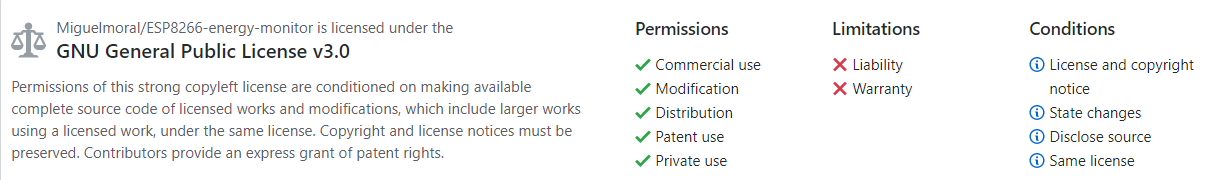
\includegraphics[scale=0.6]{imagenes/gnugpl.png}
	\caption[Resumen de la licencia GNU GPL v3]{Resumen de la licencia GNU GPL v3 Fuente: \cite{gitlicencia} }
	\label{fig:grafGNU}
\end{figure}

Todas las bibliotecas utilizadas para este proyecto tienen una licencia de software libre.

\section{Hardware principal utilizado en el proyecto}

En esta sección se hablará sobre el Hardware principal utilizado para realizar este proyecto.

\subsection{ESP8266}

Para la realización de este proyecto se ha decidido utilizar una Placa ESP8266 frente a otras soluciones más habituales como suele ser Arduino.

Uno de los problemas del Arduino es que carece de conexión a internet. Si necesitamos dotar a nuestro proyecto de conexión WIFI tendremos que utilizar un chip para proporcionar a nuestro Arduino de dicha conexión. Aquí es donde entra en juego el chip ESP8266 creado con la idea de ser utilizado en proyectos de IoT y poder dotar al Arduino de conexión WiFi.

En el mercado existen diferentes fabricantes de placas que integran el chip ESP8266, pero para este proyecto se va a utilizar la placa NodeMCU v2.

En 2014 salta al mercado el kit de desarrollo de código libre NodeMCU. Inicialmente se trataba únicamente de un firmware en lenguaje LUA. Pero dos meses después el proyecto se amplia y desarrollan una placa de hardware libre. Se trata de la primera versión conocida como v0.9 o V1. Estas placas cuentan con una memoria de 4 KBytes y un almacenamiento de 4 MBytes \cite{nodemcuwikipedia}. Existen actualmente tres versiones diferentes de esta placa. Todas estas versiones son muy similares de la primera a la segunda generación tan solo cambia la anchura de la placa ya que con la placa v1 se ocupaban los 10 pines que traen las protoboards de tamaño standard, la v2 soluciona este problema haciendo la placa un poco más estrecha dejando una fila de pines en cada lado de placa cuando colocamos esta en una protoboard, además de substituir el chip ESP12 para pasar a montar el nuevo chip mejorado ESP12E. Al tratarse de hardware libre cualquier compañía interesada puede fabricar las placas, en el caso de estas dos primeras versiones han sido producidas por la empresa Amica, sin embarco la v3 la ha sacado al mercado la empresa Lolin. Esta nueva versión v3 no aporta cambios sustanciales con respecto a la v1 y la v2, tan solo un puerto USB más robusto y ha utilizado uno de los pines reservados para alimentación USB para proporcionar un pin adicional de GND \cite{nodemcuversiones} .

Principalmente las ventajas que nos ofrece esta placa son su bajo precio, su simplicidad tanto a la hora de programar como a la hora de realizar las conexiones, la posibilidad de soportar distintos lenguajes de programación como son (LUA, MicrPhython o Arduino) y sobretodo su conexión WiFi.

En la imagen (\ref{fig:nodemcu}) podemos ver todas las conexiones de las que dispone la versión v2 de la placa NodeMCU.

\begin{figure}[H]
	\centering
	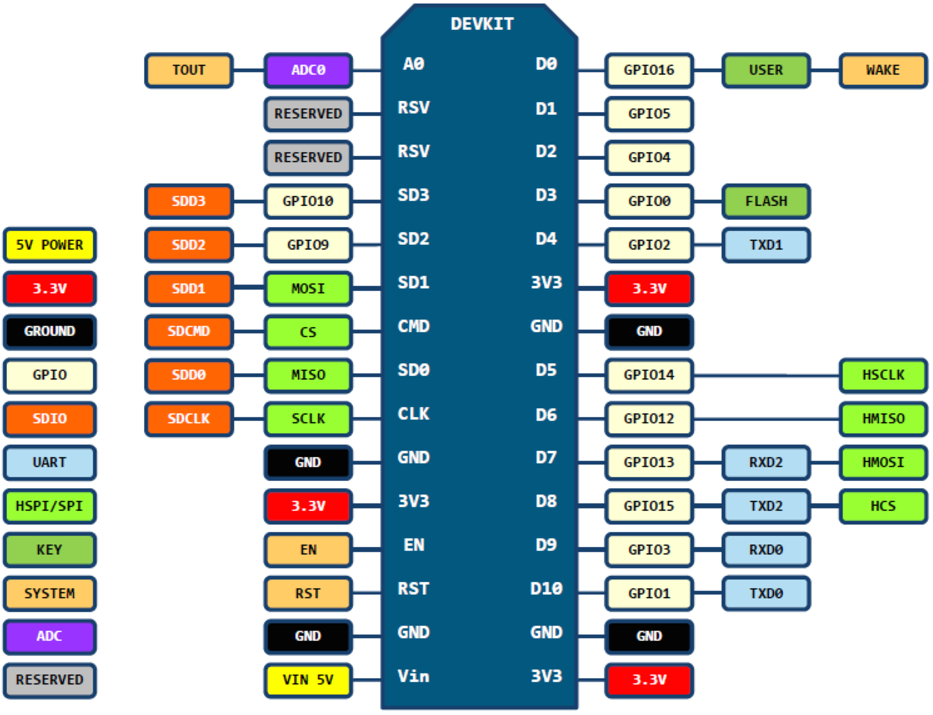
\includegraphics[scale=0.6]{imagenes/nodemcu.png}
	\caption[NodeMCU.]{NodeMCU. Fuente: \cite{nodemcuversiones}}
	\label{fig:nodemcu}
\end{figure}


\subsection{Raspberry Pi}

Se trata de una pequeña placa base que monta un procesador del fabricante Broadcom, en concreto el modelo BCM2835. Se trata de un procesador con arquitectura ARM a 1GHz de velocidad, además cuenta con una GPU VideoCore IV y una memoria de 512 MB, el almacenamiento del dispositivo dependerá la la tarjeta SD que el cliente introduzca en la placa aunque no es muy recomendable introducir SD de gran capacidad ya que las SD soportan un número limitado de lecturas y escrituras, por lo que al estar manejando un sistema operativo estas SD no suelen tener un tiempo de vida muy largo debido a la cantidad de lecturas y escrituras que tienen que realizar. Además con lo que al almacenamiento se refiere la Raspberry soporta tanto discos duros externos como pendrives por lo que el almacenamiento en este dispositivo no es ningún problema \cite{raspberrywikipedia}.

Con respecto al software podemos escoger entre una gran cantidad de sistemas operativos los cuales están disponibles para esta placa. Los más populares están basados en GNU/Linux como pueden ser Raspbian tanto su versión Lite sin entorno gráfico más dedicada al uso como servidor o su versión de escritorio una versión específica para raspberry derivada de Debian. Estos sistemas operativos se pueden descargar completamente gratis de la web oficial \cite{raspbianoficial}. Una vez descargados tan solo tendremos que flashearlos en una tarjeta SD y tendremos el sistema operativo elegido funcionando sin ningún tipo de problema en nuestra raspberry. Existen además otros sistemas operativos para esta placa permitiendo utilizarla no solo como un pequeño ordenador o como un servidor, gracias a sistemas operativos como OpenELEC podremos utilizar este dispositivo como un centro multimedia, incluso existen sistemas operativos para emular videojuegos.

Además de su reducido precio para la gran potencia que nos ofrece, una de las mayores virtudes de esta placa es el gran número de conexiones que nos ofrece. Esta placa cuenta con las siguientes conexiones (modelo Pi 2) : \cite{raspberrywikipedia}

\begin{itemize}
	\item\textbf{Puertos USB: } Dispone de 4 puertos USB 2.0.
	\item\textbf{Salidas de video: } Conector RCA, HDMI e interfaz DSI para conectar un panel LCD.
	\item\textbf{Salidas de audio: } Cuenta con un conector Jack de 3,5mm y una salida HDMI.
	\item\textbf{Conectividad de red: } Dispone de una entrada Ethernet (RJ-45).
	\item\textbf{Alimentación: } Integra una entrada microUSB de 5V para poder alimentar la placa de manera sencilla.
\end{itemize}

En la imagen (\ref{fig:Raspberryimg}) podremos ver todas las conexiones de manera más clara.

\begin{figure}[H]
	\centering
	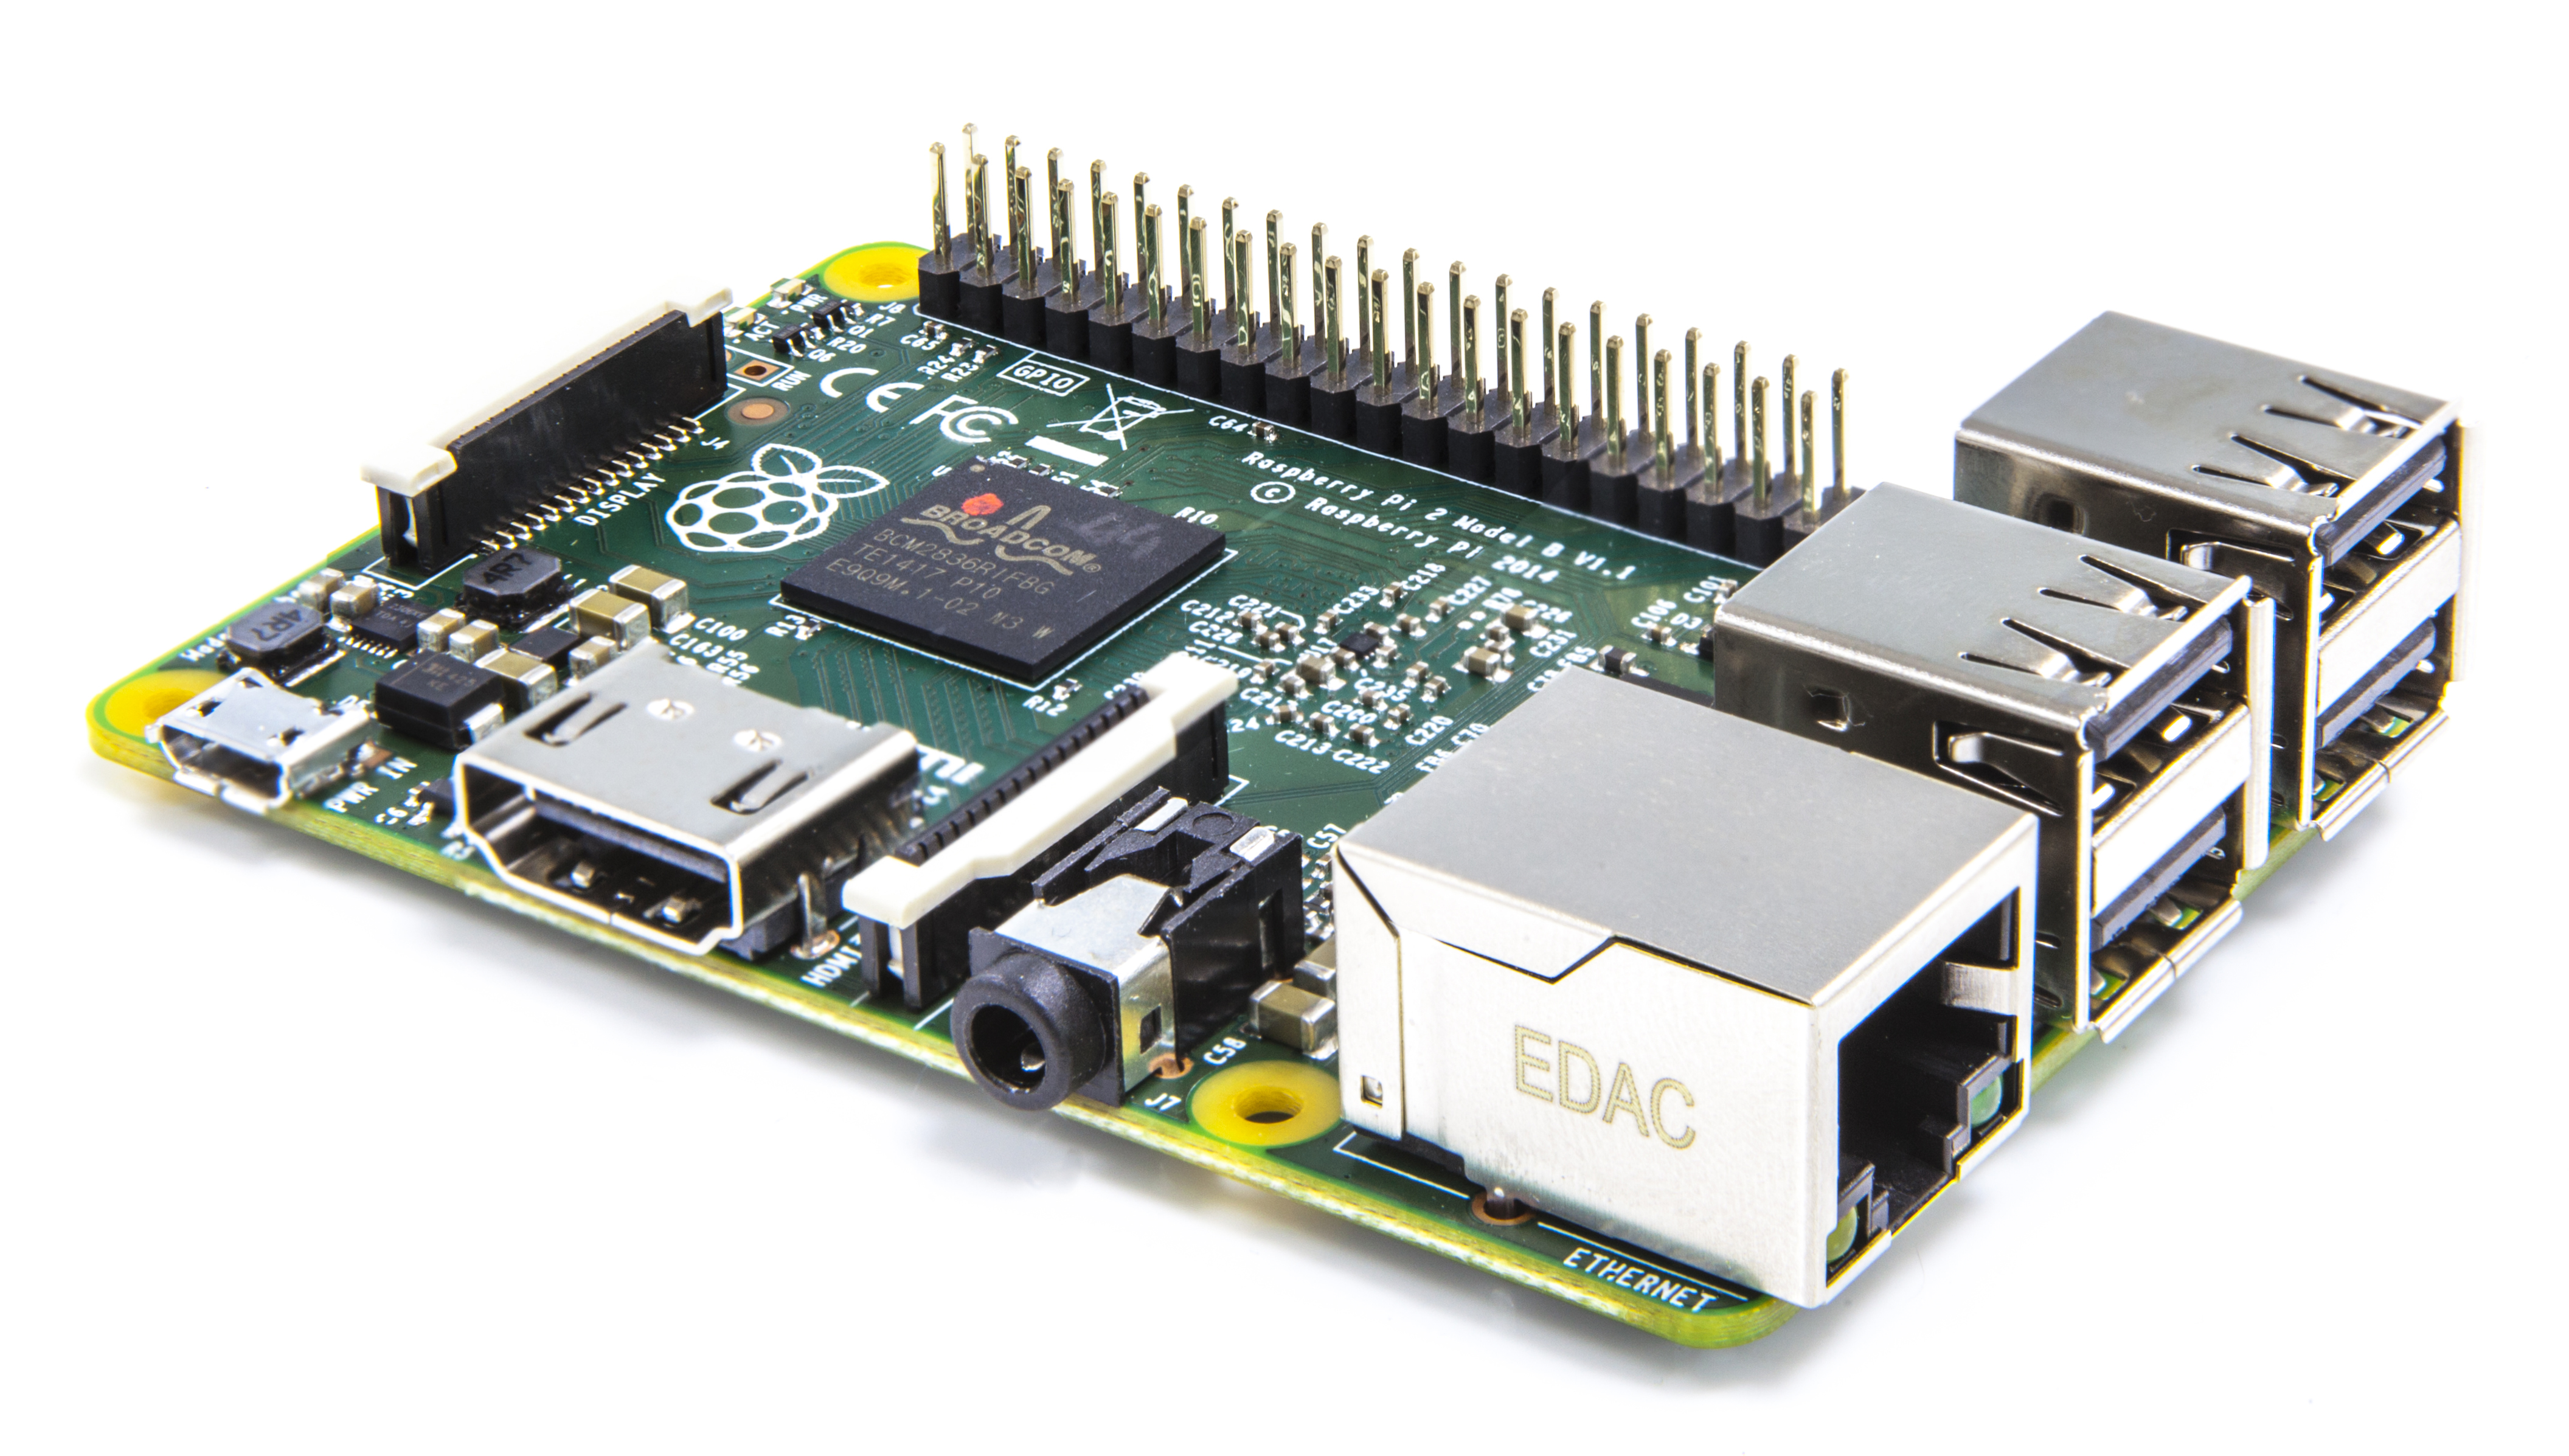
\includegraphics[scale=0.4]{imagenes/raspberry.jpg}
	\caption[Raspberry.]{Raspberry. Fuente: \cite{imagenraspberry}}
	\label{fig:Raspberryimg}
\end{figure}



\section{Sensores de energía en el mercado actual.}
Antes de empezar el proyecto es necesario analizar las soluciones que nos ofrece el mercado actualmente. A continuación vamos a repasar los puntos fuertes y los puntos débiles de estas soluciones.

\begin{itemize}
\item\textbf{Efergy Technologies ENGAGE HUB 1.1: } Se trata de un sensor que se conecta de forma inalámbrica con sus propios servidores donde se almacenará la información que se recoja en nuestro hogar. Pone a disposición del cliente un portal web gratuito que le permitirá consultar los datos recogidos, cuenta además con una aplicación para android y para IOS.Este dispositivo permite conectar una pantalla externa de la propia marca la cuál no está incluida en el precio. A un precio de 112,08 \$ (\EUR{99,9}).\cite{Efergy}
	
\begin{figure}[H]
	\centering
	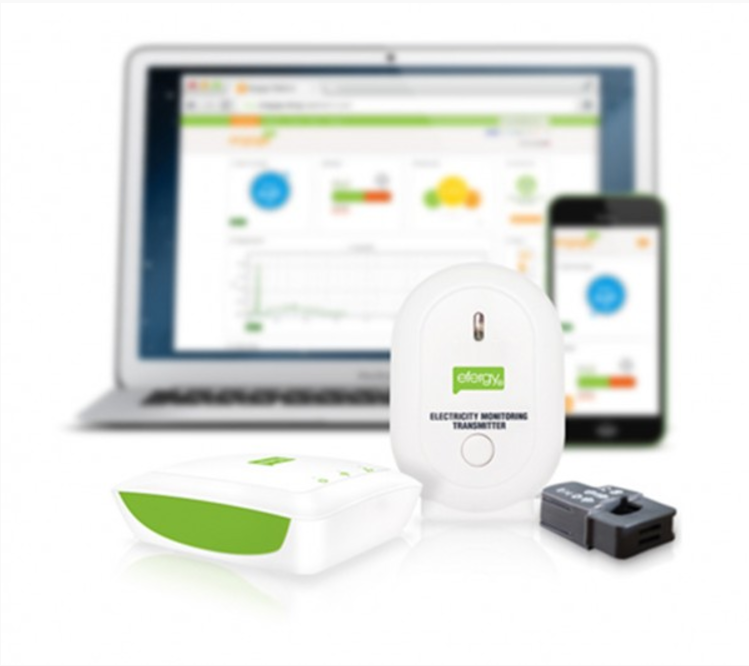
\includegraphics[scale=0.9]{imagenes/efergy.png}
	\caption[Efergy ENGAGE HUB 1.1]{Efergy ENGAGE HUB 1.1. Fuente: \cite{Efergy}}
	\label{fig:Efergy}
\end{figure}


\item\textbf{Neurio W1-HEM Home Energy Monitor: } Ofrece actualización de los datos segundo a segundo. Infraestructura basada en la nube permitiendo acceder a los datos desde cualquier lugar y aplicaciones web y para dispositivos android e IOS. Una de las ventajas de este dispositivo es que cuenta con una API pública que nos permitirá incorporar los datos que recojamos de forma sencilla. Precio en Amazon EEUU 219,99 \$. \cite{Neur}
	
	
\begin{figure}[H]
	\centering
	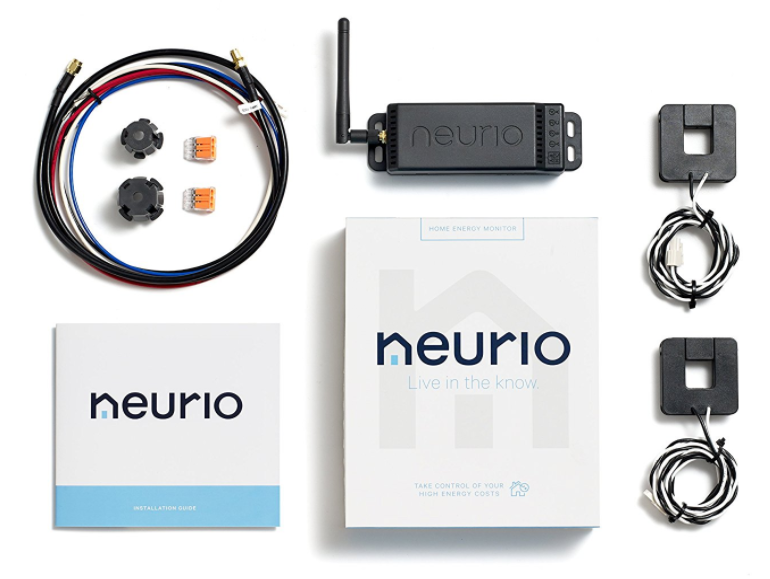
\includegraphics[scale=0.7]{imagenes/neurio.png}
	\caption[Neurio W1-HEM energy monitor]{Neurio W1-HEM energy monitor. Fuente: \cite{Neur}}
	\label{fig:neurio}
\end{figure}

\item\textbf{Efergy Technologies Elite Classic: } Es el modelo más básico de la compañía Efergy. Cuenta con una pequeña pantalla en blanco y negro que permite consultar los datos que recoge del sensor. La información que se recoge del sensor se actualiza cada 10 segundos por defecto pudiendo configurarlo para que se produzca cada 15 o 20 segundos. Este modelo no permite enviar datos a la nube, a no ser que compremos el accesorio engage. Precio de 61,50 \$ (\EUR{54,90}).\cite{Efergyclassic}

\begin{figure}[H]
	\centering
	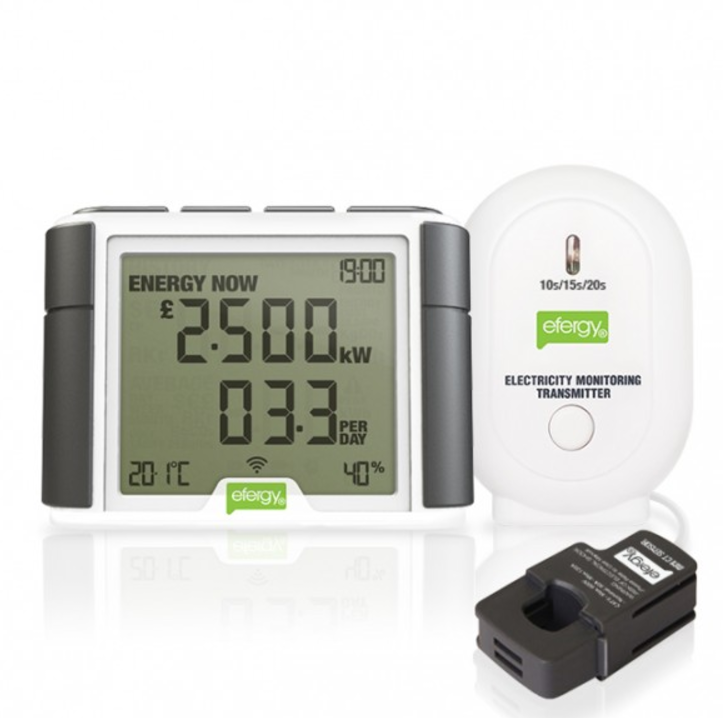
\includegraphics[scale=0.9]{imagenes/efergyclassic.png}
	\caption[Efergy Elite Classic.]{Efergy Elite Classic. Fuente: \cite{Efergyclassic}}
	\label{fig:Efergyclassic}
\end{figure}

\item\textbf{Floureon Power Meter Energy Monitor US TS-836A: } Se trata del modelo más básico de todos los que estamos analizando, siendo además el más económico de todos. Este dispositivo no se puede considerar directamente como IoT ya que tan solo muestra sus datos mediante una pantalla incorporada en el dispositivo, pero no existe la posibilidad de transmitir estos datos. Otro inconveniente de este dispositivo es que no permite monitorizar toda la casa ya que este dispositivo ha de conectarse en un enchufe. Su precio es de 20 \$ (\EUR{17,80}) más envío.\cite{floureon}

\begin{figure}[H]
	\centering
	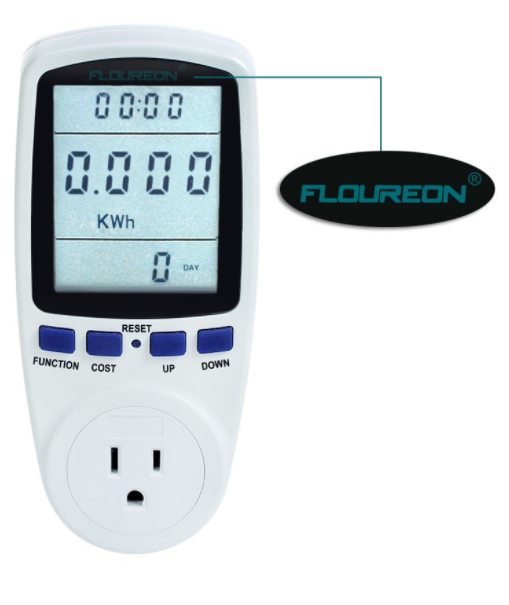
\includegraphics[scale=0.9]{imagenes/floureon.png}
	\caption[Floureon Power Meter Energy Monitor.]{Floureon Power Meter Energy Monitor. Fuente: \cite{floureon}}
	\label{fig:floureon}
\end{figure}

\item\textbf{Belkin Conserve Insight: } Se trata de un dispositivo muy similar al Floureon. La principal diferencia la encontramos en que el dispositivo de la marca Belkin nos muestra además la cantidad de dióxido de carbono que producimos según el consumo eléctrico que esté midiendo el aparato, aunque realmente se trata de una simple multiplicación. Cabe mencionar que algunos usuarios informan que la calidad de este aparato no es buena, llegando algunos usuarios incluso a comentar que el dispositivo se les ha quemado con el consiguiente riesgo de incendio. Al igual que pasaba con el dispositivo de la marca Floureon no se nos ofrece la posibilidad de almacenar los datos que recoge el sensor en ningún servidor ya que el aparato no dispone de conectividad para poder comunicarse con el servidor. El precio de este aparato es de 29,99 \$ (\EUR{26,70}). \cite{Belkin}

\begin{figure}[H]
	\centering
	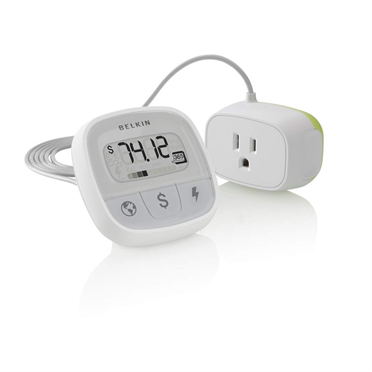
\includegraphics{imagenes/belkin.jpg}
	\caption[Belkin Conserve Insight.]{Belkin Conserve Insight. Fuente: \cite{Belkin}}
	\label{fig:Belkin}
\end{figure}

\item\textbf{EmonTx V3: } La propuesta opensource que nos trae OpenEnergyMonitor nos permitirá conectar un total de 4 sensores de energía no invasivos. Conectividad vía RF 433/868 MHz o posibilidad de dotar al aparato con conectividad WiFi utilizando una placa ESP8266. Incorpora la opción de hacer medidas de temperatura además de hacer una monitorización de energía. Permite enviar los datos recogidos por el sensor mediante RF 433/868 MHz a una raspberry o a cualquier servidor en caso de utilizar la conexión WiFi del ESP8266. A un precio de \EUR{65}.\cite{emonTx}

\begin{figure}[H]
	\centering
	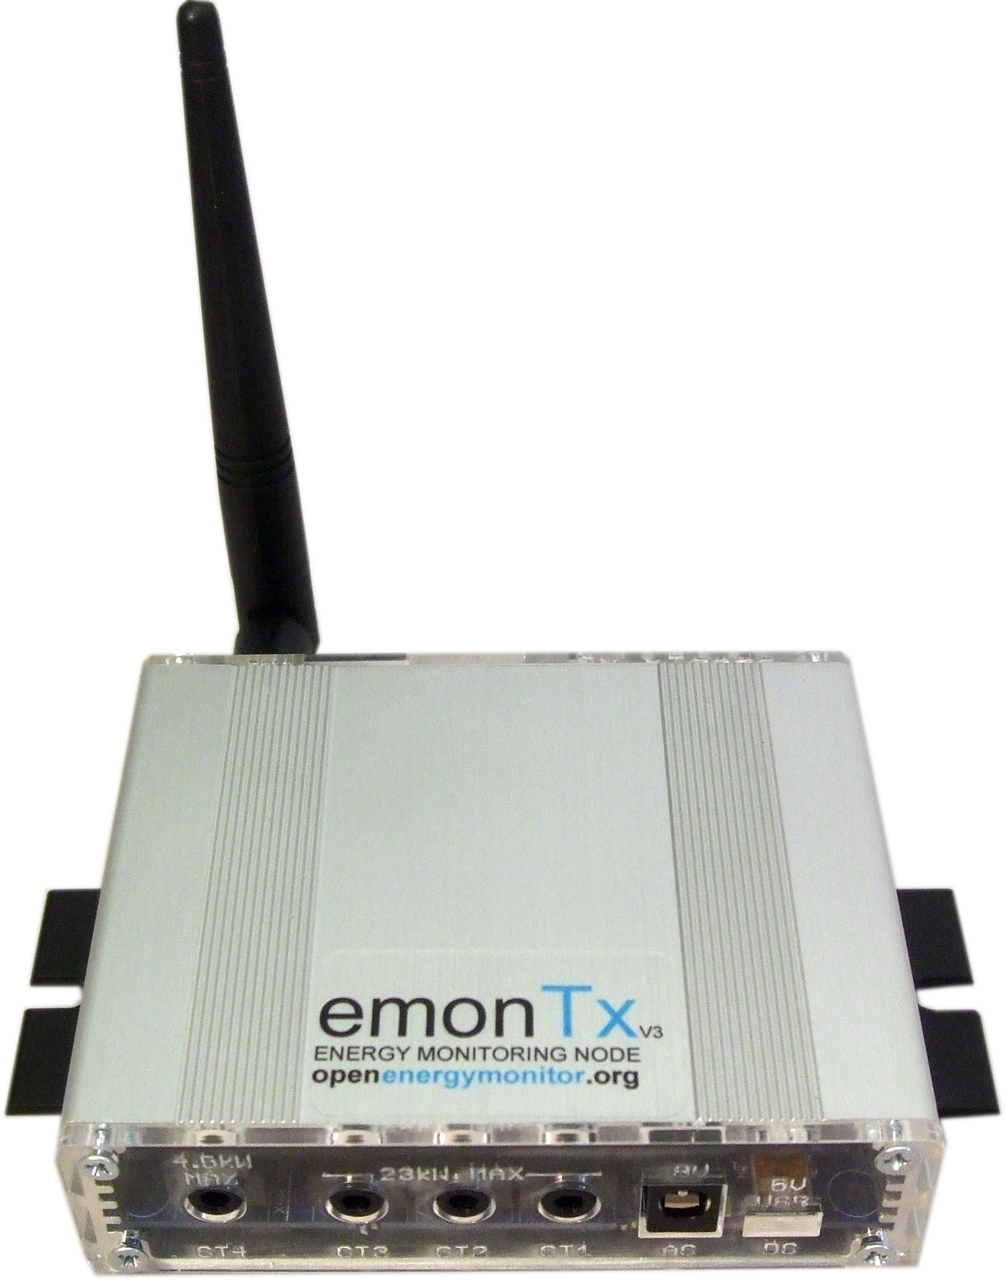
\includegraphics[scale=0.25]{imagenes/emonTx.png}
	\caption[EmonTx V3.]{EmonTx V3. Fuente: \cite{emonTx}}
	\label{fig:emonTx}
\end{figure}

\item\textbf{Sense home energy system: } Este sensor tiene como idea que nuestra casa se comunique con nosotros. De modo que la casa nos dirá durante cuanto tiempo hemos estado viendo la televisión, o durante cuanto tiempo ha estado encendida una bombilla. Este sistema no tiene que aprender nuestros hábitos durante un periodo de tiempo para reconocer que aparato está consumiendo electricidad en cada momento si no que ya conoce el modelo de consumo eléctrico de ciertos electrodomésticos y aparatos eléctricos de la casa. Este aparato se comunica mediante WiFi para mandar la información que recogen sus sensores a un servidor de la propia empresa. Podremos visualizar nuestros consumos y demás datos a través de un portal web o mediante una app disponible para Android e IOS. El precio de este producto ronda los \EUR{265}.\cite{Senseoficial}

\begin{figure}[H]
	\centering
	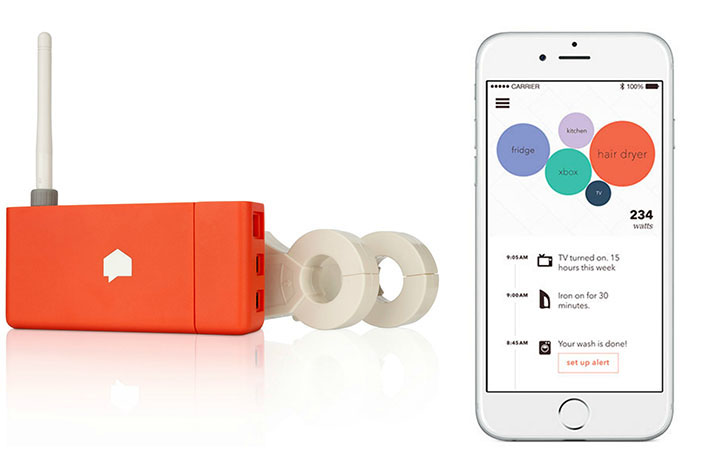
\includegraphics[scale=0.5]{imagenes/sense.jpg}
	\caption[Sense.]{Sense. Fuente: \cite{Senseimagen}}
	\label{fig:emonTx}
\end{figure}

\item\textbf{British Gas energy monitor: } Debido a una iniciativa por parte del gobierno de gran bretaña que busca reducir el consumo eléctrico de los hogares la compañía de luz y gas británica British gas podrán pedir un monitor de energía y gas de forma gratuita incluyendo su instalación. Los datos recogidos por el sensor se mandan monitor utilizando Zigbee y estos datos se mandan directamente vía GPRS a la compañía British Gas haciendo que no se tengan que revisar los consumos de cada casa ya que se actualizan automáticamente. Actualmente este dispositivo tan solo se puede conseguir siendo cliente de la compañía British Gas. \cite{BritishGas}

\begin{figure}[H]
	\centering
	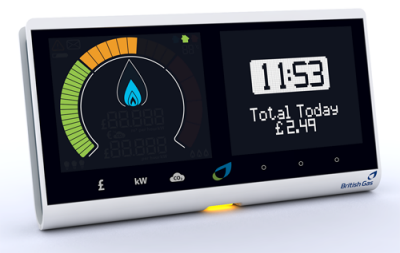
\includegraphics[scale=0.7]{imagenes/britishgas.png}
	\caption[British Gas.]{British Gas. Fuente: \cite{BritishGas}}
	\label{fig:britishgas}
\end{figure}

	
\end{itemize}




\section{Tabla comparativa de sensores de energía en el mercado.}
Mediante la tabla (\ref{tabla:monitores}) se pretende resumir de forma más clara y sencilla toda la información dada en la sección anterior de cada uno de los dispositivos que se nombraron.

\begin{landscape}
	
	\begin{table}
	
			\resizebox{25cm}{!} {
				\begin{tabular}{|l||c|c|c|c|c|c|c|c|c|}
					\hline
					Modelo & Dispone API & Tiempo refresco & Protocolo Comunicación & Monitorización solar & Pantalla para visualizar datos & Cloud & Precio\EUR{} \\
					\hline \hline 
					Efergy Engage & \checkmark & Seleccionable 10, 15 o 20 sec & Wifi & Con accesorio & Con módulo Elite classic & \checkmark & 99.9\\ \hline
					Efergy elite  & \checkmark & Seleccionable 10, 15 o 20 sec & Sin especificar & Con accesorio & \checkmark & Con módulo Engage & 195.86\\ \hline
					Neurio & \checkmark & Instantáneo & Wifi 802.1 b/n/g & Con accesorio & $\times$ & \checkmark & 54.90\\ \hline
					Floureon & $\times$ & Instantáneo & No transmite datos & $\times$ & \checkmark & $\times$ & 17.80\\ \hline
					Belkin & $\times$ & Instantáneo & No transmite datos & $\times$ & \checkmark & $\times$ & 26.70\\ \hline
					EmonTx V3 & $\times$ & Instantáneo & RF 433/868 MHz & $\times$ & \checkmark & \checkmark & 65\\ \hline
					Sense & $\times$ & Instantáneo & Wifi, Bluetooth & Con accesorio & $\times$ & \checkmark & 265\\ \hline
					British Gas & $\times$ & Instantáneo & GPRS, Zigbee & $\times$ & \checkmark & \checkmark & -\\ \hline
				\end{tabular}
			}
			\caption{Monitores de energía en el mercado.}
			\label{tabla:monitores}
	\end{table}

\end{landscape}

Teniendo en cuenta las diferencias entre modelos y los precios de cada aparato existen dos alternativas principales en función de la necesidad del cliente las mejores opciones serían :

\begin{itemize}
	\item\textbf{Monitorizar el consumo de un solo electrodoméstico: } En caso de que el cliente necesite un dispositivo sencillo al menor precio posible, recomendaría el dispositivo de la marca Belkin  (Conserve Insight). Si lo comparamos frente a su competidor el Floureon la diferencia de precio es de tan solo unos 9 euros permitiéndonos el dispositivo de la marca Belkin visualizar la cantidad de dióxido de carbono que producimos. Por lo demás ambos dispositivos son muy similares.
	\item\textbf{Monitorizar el consumo de toda la casa: } Como podemos observar en el caso de querer monitorizar la casa entera el precio de los dispositivos se dispara. En mi opinión el mejor dispositivo de los que se han presentado es el Efergy Technologies Elite Classic, además de ser el más económico de los tres modelos que permiten monitorizar el consumo de toda la casa podremos actualizar el dispositivo y comprar el módulo Engage para almacenar nuestros datos en los servidores que nos brinda la empresa Efergy y poder visualizar nuestros consumos desde su plataforma web o sus aplicaciones para dispositivos móviles. No considero que sea rentable pagar la diferencia de precio existente con el modelo que nos ofrece la compañia Neurio ya que no existen diferencias que justifiquen este sobreprecio. Sin embargo la característica que nos trae Sense que nos permite comunicarnos con nuestra casa viendo consumos exclusivos de cada aparato me parece muy interesante aunque en mi opinión no justifica el alto precio del producto.El EmonTx no me parece mala opción pero es necesario documentarse un poco para poder empezar a utilizarlo si no se tiene experiencia.
	
\end{itemize}

\section{Porqué hacer nuestro propio monitor}

Como podemos observar en el mercado existen diversas propuestas que se pueden adaptar a las necesidades que buscamos cubrir, pero en este proyecto se va a llevar a cabo el diseño y construcción de un monitor con características similares a los que existen. Algunos de los motivos que nos han llevado a realizar nuestro propio monitor son los siguientes:

\begin{itemize}
	\item\textbf{Aprender: } Durante todo el proceso se van a adquirir conocimientos en diversas áreas como pueden ser hardware, electrónica, etc.
	\item\textbf{Precios: } Podremos además comprobar si el precio de realizar nuestro propio dispositivo es razonable con respecto a los precios que nos ofrecen aparatos comerciales.
	\item\textbf{No usar servicios externos: } A la hora de enviar los datos recogidos con nuestro dispositivo tendremos total libertad de escoger en que servidor se van a almacenar estos, pudiendo ser tanto un servidor local como cualquier otro servidor.
\end{itemize}
